% Reproduzierbare Vektorquelle für das gleichnamige PDF in Images/.
% Aus dem Repository-Wurzelverzeichnis bauen:
% latexmk -pdf -halt-on-error -interaction=nonstopmode \
%   -outdir=build/figures \
%   Images/sources/hash-table-linear-probing-collisions.tex
% cp build/figures/hash-table-linear-probing-collisions.pdf Images/
\documentclass[tikz,border=1pt]{standalone}

\usepackage{cmap}
\usepackage[T1]{fontenc}
\usepackage[scaled=0.95]{helvet}
\renewcommand{\familydefault}{\sfdefault}
\usetikzlibrary{arrows.meta}
\usetikzlibrary{calc}

\definecolor{DiagramNavy}{RGB}{23,54,93}
\definecolor{DiagramGray}{RGB}{127,140,141}
\definecolor{DiagramLightBlue}{RGB}{220,234,247}
\definecolor{DiagramMidBlue}{RGB}{141,185,226}
\definecolor{DiagramOrange}{RGB}{237,125,49}
\definecolor{DiagramPeach}{RGB}{252,228,214}
\definecolor{DiagramGreen}{RGB}{112,173,71}
\definecolor{DiagramLightGreen}{RGB}{217,234,211}
\definecolor{DiagramNearWhite}{RGB}{242,242,242}
\definecolor{DiagramRule}{RGB}{217,226,243}
\definecolor{DiagramRed}{RGB}{192,57,43}

\begin{document}
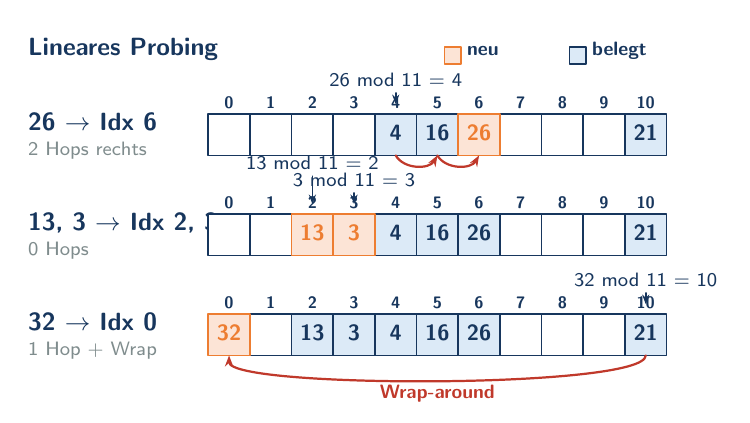
\begin{tikzpicture}[x=1bp,y=1bp,line cap=round,line join=round]
  \path[use as bounding box] (0,-14) rectangle (250,118);
  \fill[white] (0,-14) rectangle (250,118);

  \tikzset{
    heading/.style={anchor=base west,inner sep=0pt,text=DiagramNavy,
      font=\fontsize{8.5bp}{8.5bp}\selectfont\bfseries},
    body/.style={anchor=base west,inner sep=0pt,text=DiagramGray,
      font=\fontsize{7bp}{7bp}\selectfont},
    cellindex/.style={anchor=base,inner sep=0pt,text=DiagramNavy,
      font=\fontsize{6bp}{6bp}\selectfont\bfseries},
    formula/.style={anchor=base,inner sep=0pt,text=DiagramNavy,
      font=\fontsize{6.5bp}{6.5bp}\selectfont},
    legendtext/.style={anchor=base west,inner sep=0pt,text=DiagramNavy,
      font=\fontsize{7bp}{7bp}\selectfont\bfseries},
  }

  % Main Title & Legend
  \node[heading,font=\fontsize{9bp}{9bp}\selectfont\bfseries] at (0,108) {Lineares Probing};
  
  \draw[line width=0.6bp,draw=DiagramOrange,fill=DiagramPeach] (150,105) rectangle ++(6,6);
  \node[legendtext] at (158,108) {neu};
  
  \draw[line width=0.6bp,draw=DiagramNavy,fill=DiagramLightBlue] (195,105) rectangle ++(6,6);
  \node[legendtext] at (203,108) {belegt};

  % ==================== SCHRITT 1 ====================
  \node[heading] at (0,81) {26 $\rightarrow$ Idx 6};
  \node[body] at (0,72) {2 Hops rechts};

  % Cells Step 1
  \foreach \i in {0,1,2,3,7,8,9} {
    \draw[line width=0.6bp,draw=DiagramNavy,fill=white] ({65+15*\i},72) rectangle ++(15,15);
  }
  \foreach \i/\val in {4/4,5/16,10/21} {
    \draw[line width=0.6bp,draw=DiagramNavy,fill=DiagramLightBlue] ({65+15*\i},72) rectangle ++(15,15);
    \node[anchor=base,text=DiagramNavy,font=\fontsize{8bp}{8bp}\selectfont\bfseries] at ({65+15*\i+7.5},77.5) {\val};
  }
  \draw[line width=0.6bp,draw=DiagramOrange,fill=DiagramPeach] ({65+15*6},72) rectangle ++(15,15);
  \node[anchor=base,text=DiagramOrange,font=\fontsize{8bp}{8bp}\selectfont\bfseries] at ({65+15*6+7.5},77.5) {26};

  % Indices Step 1
  \foreach \i in {0,...,10} {
    \node[cellindex] at ({65+15*\i+7.5},89) {\i};
  }

  % Hash formula & Arrow Step 1
  \node[formula] at (132.5,97) {26 mod 11 = 4};
  \draw[-{Stealth[scale=0.6]},line width=0.6bp,draw=DiagramNavy] (132.5,94.5) -- (132.5,90.5);

  % Probing arrows Step 1
  \draw[-{Stealth[scale=0.6]},line width=0.8bp,draw=DiagramRed] (132.5,72) to[out=-60,in=-120] (147.5,72);
  \draw[-{Stealth[scale=0.6]},line width=0.8bp,draw=DiagramRed] (147.5,72) to[out=-60,in=-120] (162.5,72);


  % ==================== SCHRITT 2 ====================
  \node[heading] at (0,45) {13, 3 $\rightarrow$ Idx 2, 3};
  \node[body] at (0,36) {0 Hops};

  % Cells Step 2
  \foreach \i in {0,1,7,8,9} {
    \draw[line width=0.6bp,draw=DiagramNavy,fill=white] ({65+15*\i},36) rectangle ++(15,15);
  }
  \foreach \i/\val in {4/4,5/16,6/26,10/21} {
    \draw[line width=0.6bp,draw=DiagramNavy,fill=DiagramLightBlue] ({65+15*\i},36) rectangle ++(15,15);
    \node[anchor=base,text=DiagramNavy,font=\fontsize{8bp}{8bp}\selectfont\bfseries] at ({65+15*\i+7.5},41.5) {\val};
  }
  \foreach \i/\val in {2/13,3/3} {
    \draw[line width=0.6bp,draw=DiagramOrange,fill=DiagramPeach] ({65+15*\i},36) rectangle ++(15,15);
    \node[anchor=base,text=DiagramOrange,font=\fontsize{8bp}{8bp}\selectfont\bfseries] at ({65+15*\i+7.5},41.5) {\val};
  }

  % Indices Step 2
  \foreach \i in {0,...,10} {
    \node[cellindex] at ({65+15*\i+7.5},53) {\i};
  }

  % Hash formulas Step 2 (staggered above cells to avoid overlaps)
  \node[formula] at (117.5,61) {3 mod 11 = 3};
  \draw[-{Stealth[scale=0.6]},line width=0.6bp,draw=DiagramNavy] (117.5,58.5) -- (117.5,54.5);

  \node[formula] at (102.5,67) {13 mod 11 = 2};
  \draw[-{Stealth[scale=0.6]},line width=0.6bp,draw=DiagramNavy] (102.5,64.5) -- (102.5,54.5);


  % ==================== SCHRITT 3 ====================
  \node[heading] at (0,9) {32 $\rightarrow$ Idx 0};
  \node[body] at (0,0) {1 Hop + Wrap};

  % Cells Step 3
  \foreach \i in {1,7,8,9} {
    \draw[line width=0.6bp,draw=DiagramNavy,fill=white] ({65+15*\i},0) rectangle ++(15,15);
  }
  \foreach \i/\val in {2/13,3/3,4/4,5/16,6/26,10/21} {
    \draw[line width=0.6bp,draw=DiagramNavy,fill=DiagramLightBlue] ({65+15*\i},0) rectangle ++(15,15);
    \node[anchor=base,text=DiagramNavy,font=\fontsize{8bp}{8bp}\selectfont\bfseries] at ({65+15*\i+7.5},5.5) {\val};
  }
  \draw[line width=0.6bp,draw=DiagramOrange,fill=DiagramPeach] ({65+15*0},0) rectangle ++(15,15);
  \node[anchor=base,text=DiagramOrange,font=\fontsize{8bp}{8bp}\selectfont\bfseries] at ({65+15*0+7.5},5.5) {32};

  % Indices Step 3
  \foreach \i in {0,...,10} {
    \node[cellindex] at ({65+15*\i+7.5},17) {\i};
  }

  % Hash formula Step 3
  \node[formula] at (222.5,25) {32 mod 11 = 10};
  \draw[-{Stealth[scale=0.6]},line width=0.6bp,draw=DiagramNavy] (222.5,22.5) -- (222.5,18.5);

  % Probing / Wrap-around arrow Step 3
  \draw[-{Stealth[scale=0.6]},line width=0.8bp,draw=DiagramRed] (222.5,0) .. controls (222.5,-12) and (72.5,-12) .. (72.5,0);
  \node[text=DiagramRed,font=\fontsize{6.5bp}{6.5bp}\selectfont\bfseries,anchor=north] at (147.5,-7) {Wrap-around};

\end{tikzpicture}
\end{document}
